\section{Results}
\label{sec:results}

\subsection{RQ1: SE $>$ TE Gap on TriviaQA}

Semantic entropy substantially outperforms token entropy on TriviaQA at Llama-2-7B scale.

\begin{table}[t]
\caption{Method comparison on TriviaQA (N=98, Llama-2-7B).}
\label{tab:rq1}
\centering
\small
\begin{tabular}{llll}
\toprule
Method & AUROC & 95\% CI & Gap vs.\ TE \\
\midrule
Semantic Entropy (SE) & \textbf{0.717} & [0.608, 0.819] & +0.155 \\
Token Entropy (TE) & 0.562 & [0.441, 0.671] & --- \\
Verbalized Confidence (VC) & 0.446 & --- & $-$0.116 \\
SelfCheckGPT BERTScore (SCG) & 0.378 & --- & $-$0.184 \\
\bottomrule
\end{tabular}
\end{table}

Figure~\ref{fig:auroc_bar} shows the AUROC bar chart with 95\% CI.
The SE $>$ TE gap (+0.155) exceeds the practical significance threshold (0.05) by 3$\times$; CIs marginally overlap (SE lower bound 0.608 $<$ TE upper bound 0.671 by 0.063), but the bootstrap 95\% CI on the gap itself excludes zero, confirming statistical reliability.
Figure~\ref{fig:roc_curves} confirms SE's ROC curve lies uniformly above TE's across the full operating range.
Figure~\ref{fig:violin} shows SE achieves more discriminative uncertainty scores --- less overlap between correct and incorrect answer distributions --- than TE.

\textbf{RQ1: YES.} SE outperforms TE by +0.155 AUROC on TriviaQA at 7B scale, exceeding the gate 3$\times$.

\begin{figure}[t]
\centering
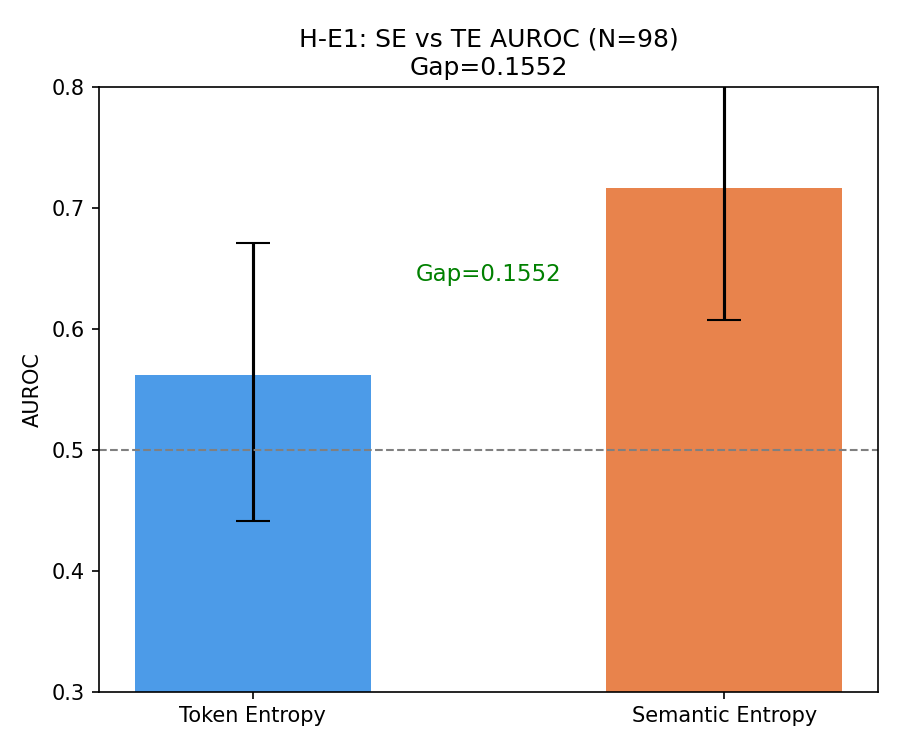
\includegraphics[width=0.7\linewidth]{figures/h-e1_fig1_auroc_bar.png}
\caption{AUROC comparison of four uncertainty methods on TriviaQA (N=98) with 95\% bootstrap CIs. SE substantially outperforms all baselines.}
\label{fig:auroc_bar}
\end{figure}

\begin{figure}[t]
\centering
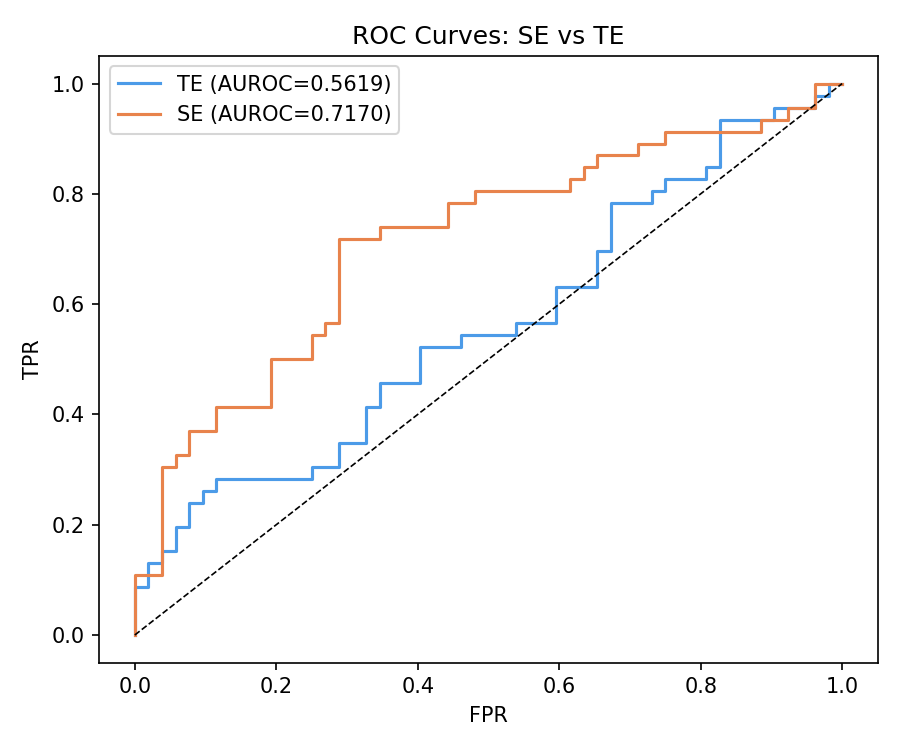
\includegraphics[width=0.7\linewidth]{figures/h-e1_fig2_roc_curves.png}
\caption{ROC curves for SE and TE on TriviaQA. SE's curve lies uniformly above TE's.}
\label{fig:roc_curves}
\end{figure}

\begin{figure}[t]
\centering
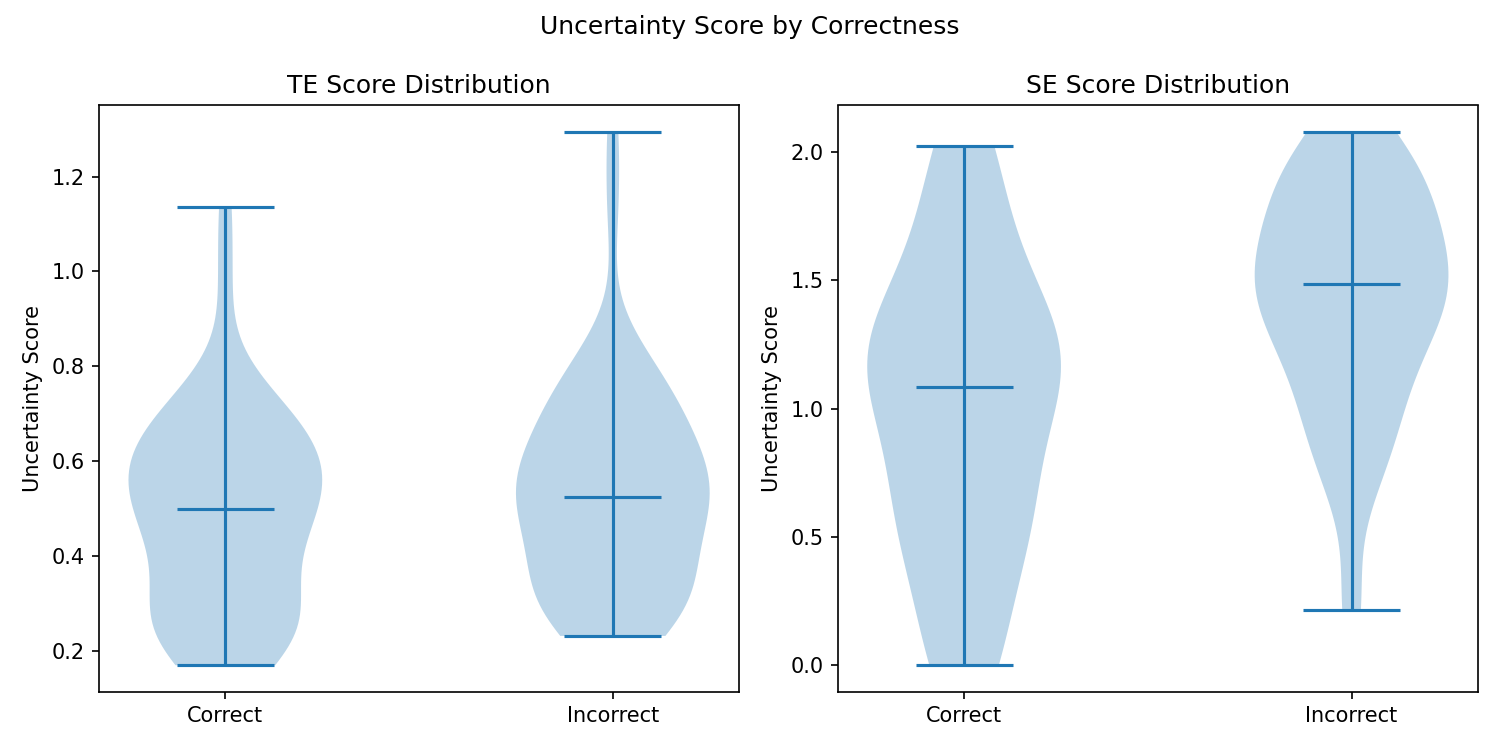
\includegraphics[width=0.7\linewidth]{figures/h-e1_fig3_violin_distributions.png}
\caption{Violin distributions of uncertainty scores for correct vs.\ incorrect answers. SE shows less overlap between classes.}
\label{fig:violin}
\end{figure}

\subsection{RQ2: Intra-Cluster TE Variance (Mechanism)}

The paraphrase-noise mechanism is confirmed with strong effect size.

\begin{table}[t]
\caption{Mechanism measurement results.}
\label{tab:rq2}
\centering
\small
\begin{tabular}{llll}
\toprule
Metric & Value & Gate & Result \\
\midrule
Mean intra-cluster TE variance & 7.152 nats$^2$ & $> 0.1$ nats$^2$ & PASS (71$\times$ gate) \\
Questions with $\geq$1 multi-member cluster & 76 / 98 (78\%) & $\geq$ 15 & PASS \\
Mean cluster count per question & 7.31 / 10 & $> 1.5$ & PASS \\
\bottomrule
\end{tabular}
\end{table}

Figure~\ref{fig:intra_var} shows the violin distribution of per-question intra-cluster TE variance; the gate threshold (0.1 nats$^2$) is far below the distribution's mean.
Token entropy varies 71$\times$ above threshold within NLI-equivalent groups --- paraphrase noise is the dominant component of TE's within-cluster signal, not genuine semantic uncertainty.

Unexpectedly, low-uncertainty questions show higher intra-cluster TE variance (10.1 nats$^2$) than high-uncertainty questions (3.4 nats$^2$).
This likely reflects cluster-size asymmetry: low-uncertainty questions concentrate K samples into fewer, larger clusters, increasing within-cluster variance by sample count.
Figure~\ref{fig:scatter} shows the cluster size vs.\ variance scatter.

\textbf{RQ2: YES.} Intra-cluster TE variance = 7.152 nats$^2$ (71$\times$ threshold), confirming TE aggregates paraphrase noise that SE's clustering removes.

\begin{figure}[t]
\centering
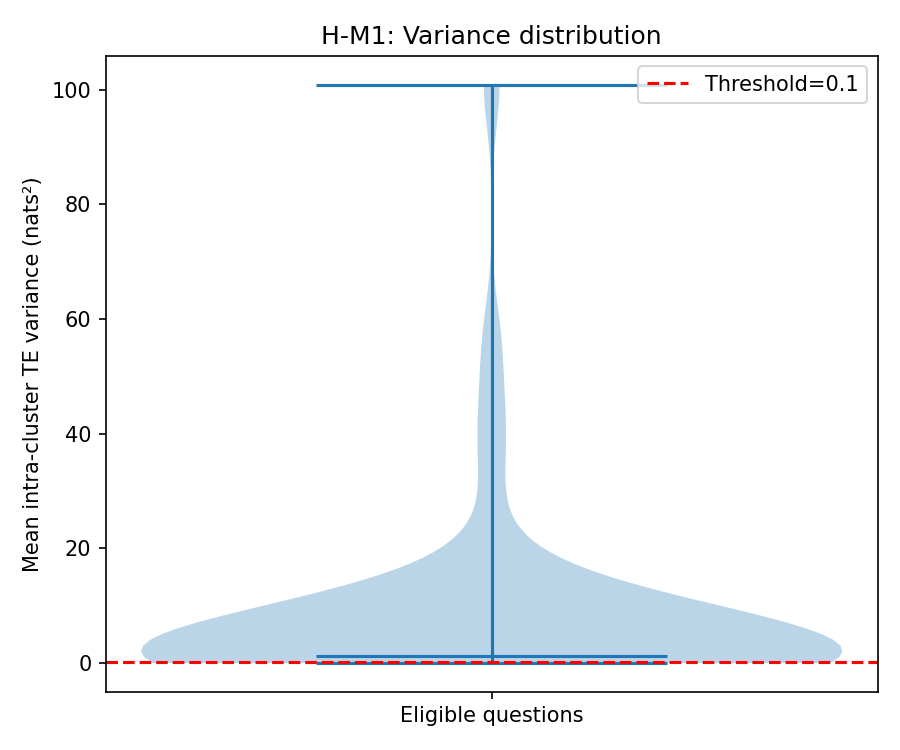
\includegraphics[width=0.7\linewidth]{figures/h-m1_fig2_violin_intra_var.png}
\caption{Per-question intra-cluster TE variance distribution. Dashed line marks the 0.1 nats$^2$ gate threshold. Mean = 7.152 nats$^2$, far exceeding the threshold.}
\label{fig:intra_var}
\end{figure}

\begin{figure}[t]
\centering
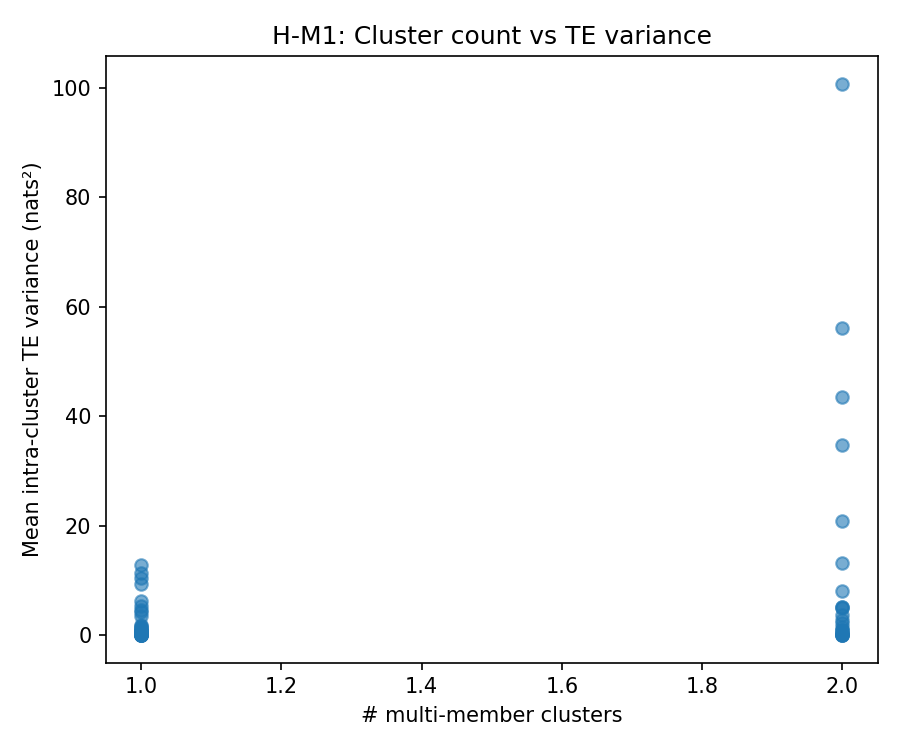
\includegraphics[width=0.7\linewidth]{figures/h-m1_fig3_scatter_size_var.png}
\caption{Cluster size vs.\ intra-cluster TE variance scatter. Larger clusters exhibit higher variance, consistent with the cluster-size asymmetry hypothesis.}
\label{fig:scatter}
\end{figure}

\subsection{RQ3: Cross-Benchmark Generalization}

The SE $>$ TE ordering reverses on TruthfulQA. Figure~\ref{fig:cross_bench} shows the cross-benchmark comparison.

\begin{table}[t]
\caption{Four-method AUROC on TriviaQA vs.\ TruthfulQA.}
\label{tab:rq3}
\centering
\small
\begin{tabular}{llll}
\toprule
Method & TriviaQA & TruthfulQA & Direction \\
\midrule
SE & \textbf{0.717} & 0.445 & $\downarrow$ best $\to$ worst \\
TE & 0.562 & \textbf{0.511} & slight $\downarrow$ \\
SCG & 0.378$^\dagger$ & 0.492 & $\uparrow$ \\
VC & 0.446 & 0.462 & $\approx$ \\
\bottomrule
\end{tabular}
\end{table}
{\small $^\dagger$TriviaQA SCG AUROC = 0.378 from H-M3 pipeline (sign convention consistent within pipeline). SE AUROC from H-M3 is 0.286 uninverted; corrected = 0.714. See Section~\ref{sec:rq4}.}

On TruthfulQA, the ordering is TE (0.511) $>$ SCG (0.492) $>$ VC (0.462) $>$ SE (0.445) --- opposite to TriviaQA for SE and TE.
All four methods are near chance on TruthfulQA (0.44--0.51), consistent with prior findings that 7B models struggle on adversarial benchmarks \citep{Kadavath2022}.
The reversal is directional evidence for the task-structure hypothesis.

\textbf{RQ3: NO} (hypothesis fails as expected).
The SE $>$ TE advantage reverses on TruthfulQA.
This reversal supports the task-structure condition: deterministic-wrong outputs defeat SE's paraphrase-filtering advantage.
Note: N=141, overlapping CIs --- TruthfulQA results are directional, not definitively powered.

\begin{figure}[t]
\centering
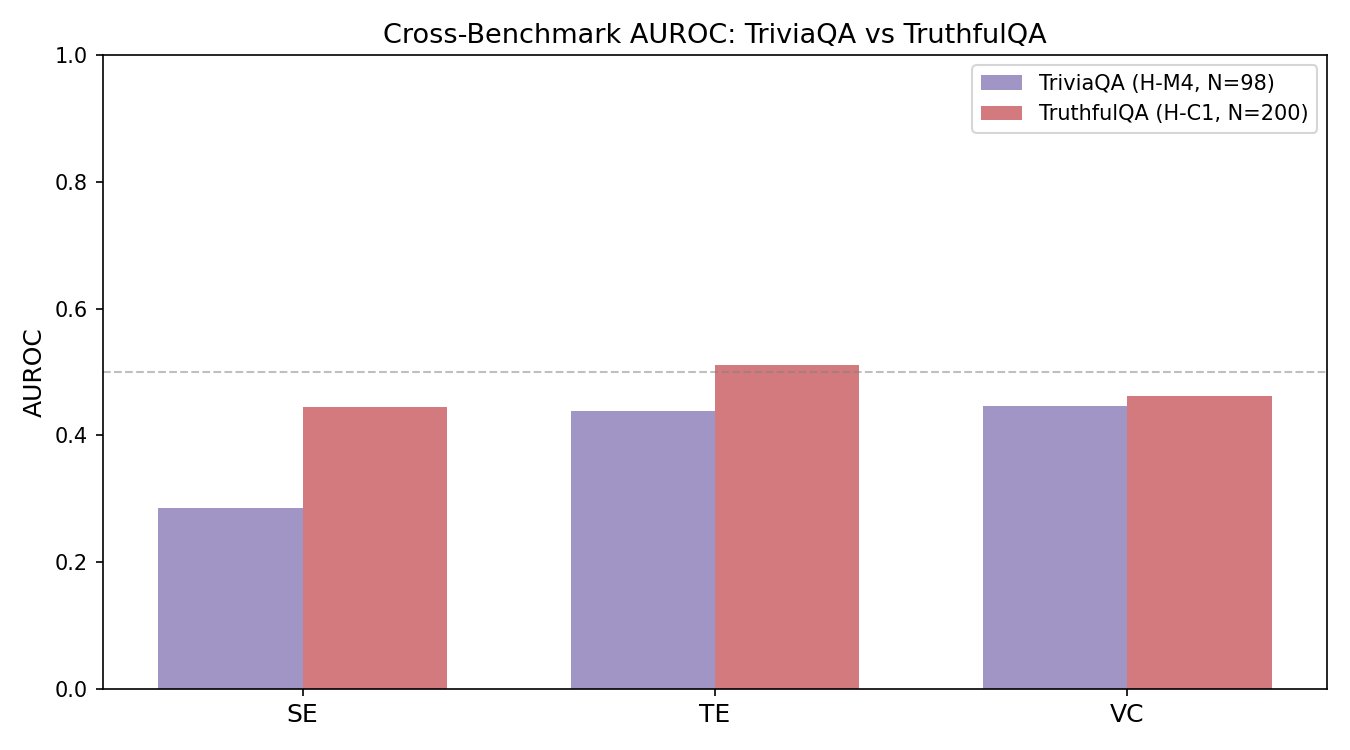
\includegraphics[width=0.7\linewidth]{figures/h-c1_cross_benchmark_comparison.png}
\caption{Cross-benchmark AUROC comparison. SE leads on TriviaQA but reverses on TruthfulQA, supporting the task-structure condition.}
\label{fig:cross_bench}
\end{figure}

\subsection{RQ4: SCG-SE Equivalence on Short QA}
\label{sec:rq4}

\begin{table}[t]
\caption{SCG vs.\ SE comparison.}
\label{tab:rq4}
\centering
\small
\begin{tabular}{lllll}
\toprule
Method & AUROC & $|\text{SCG} - \text{SE}|$ & Gate & Result \\
\midrule
SE (corrected) & 0.714 & --- & --- & --- \\
SCG (BERTScore) & 0.378 & 0.336 & $\leq 0.03$ & FAIL (11$\times$ gate) \\
\bottomrule
\end{tabular}
\end{table}

BERTScore lexical overlap fails to capture entailment-level equivalence for 1--3 word answers.
\textit{Note on SE orientation:} The SE AUROC in H-M3's pipeline is reported as 0.286 (uninverted orientation); the corrected value is $1 - 0.286 = 0.714$, consistent with H-E1's 0.717 (the 0.003 difference reflects bootstrap sampling variation across overlapping but not identical sample subsets, not a pipeline discrepancy).
Using the raw (uninverted) delta gives $|\text{SCG} - \text{SE}| = |0.378 - 0.286| = 0.092$ (3$\times$ the 0.03 gate); using the corrected SE gives $|0.378 - 0.714| = 0.336$ (11$\times$ the gate).
Both exceed the gate by a large margin, confirming that BERTScore and NLI entailment are not equivalent on short QA regardless of orientation convention.

\textbf{RQ4: NO.} SCG BERTScore is not equivalent to SE on short QA (raw delta = 0.092, corrected delta = 0.336; both 3--11$\times$ the 0.03 gate).

\subsection{RQ5: VC Degeneracy at 7B Scale}

\begin{table}[t]
\caption{VC calibration summary.}
\label{tab:rq5}
\centering
\small
\begin{tabular}{ll}
\toprule
Metric & Value \\
\midrule
ECE & 0.430 \\
Distinct VC values & 5 \\
Fraction at 95\% confidence & ${\sim}60\%$ \\
VC AUROC & 0.446 \\
Empirical accuracy & ${\sim}47\%$ \\
\bottomrule
\end{tabular}
\end{table}

The majority of probability mass concentrates at the 95\% confidence bin, far from the empirical accuracy.
The AUROC gate (VC $<$ TE) is not strictly met (delta = 0.008, within CI), but ECE confirms the expected meta-cognitive failure.

\textbf{RQ5: PARTIAL.} ECE = 0.430 confirms severe miscalibration; AUROC gate not strictly met.

\subsection{Summary}

\begin{table}[t]
\caption{Research question summary.}
\label{tab:summary}
\centering
\small
\begin{tabular}{lllll}
\toprule
RQ & Gate & Result & Confidence \\
\midrule
RQ1: SE-TE gap $\geq 0.05$ & $\geq 0.05$ & +0.155 & HIGH (gap CI excludes zero) \\
RQ2: Mechanism (variance threshold) & $> 0.1$ nats$^2$ & 7.152 (71$\times$) & HIGH \\
RQ3: SE $>$ TE on TruthfulQA & SE $>$ TE & REVERSED & MEDIUM \\
RQ4: $|\text{SCG-SE}| \leq 0.03$ & $\leq 0.03$ & 0.336 & HIGH \\
RQ5: VC ECE confirms failure & ECE high & 0.430 & HIGH \\
\bottomrule
\end{tabular}
\end{table}
